\documentclass{beamer}
\usetheme{Madrid}
\usepackage{graphicx}
\usepackage[T1]{fontenc}
% \usepackage[polish]{babel}
% \usepackage[polish]{datetime2}
\usepackage{graphicx}
\usepackage{caption}


\usepackage{tikz}
\def\checkmark{\tikz\fill[scale=0.4](0,.35) -- (.25,0) -- (1,.7) -- (.25,.15) -- cycle;} 


\title{Games classifier}

\author[Team name]{Team name\\[5mm]
{\small Members: Julia Cygan, Borys Adamiak, Patryk Flama}
\hspace{18mm} 
{\small Supervisor: Marek Adamczyk}}

\institute{UWr}
\date{\today}

\begin{document}

\begin{frame}
\titlepage
\end{frame}


\begin{frame}[t]{Goal and motivation}

{\bf Use case example:} \\
Imagine that you run a online game store where users can add their games to your library. Instead of manually checking if user tagged correctly the game, you can use our model to do that job for you. \\

\vspace{3mm}

{\bf Goal:} \\
We want to be able to automatically assign tags (or genres) to games, based on their (text) description.

\vspace{3mm}

Additionally, in aspect of ML project, we want to make a small comparison of different models and methods for solving such multilabel classification problem.
\end{frame}

\begin{frame}[t]{Info about the dataset}
Steam has its own official API, from which we downloaded games, their descriptions, tags and genres. That resulted in a bit over {\it 200'000} games. \\
\vspace{2mm}
To clean the data we:
\begin{itemize}
	\item Converted descriptions to alphanumeric lowercase
	\item Removed html tags
	\item Removed empty descriptions or tags
	\item (optional) Removed tags/genres that occured at most {\it n} times
\end{itemize}
After that we ended up with a dataset of size around {\it 50'000} games and {\it 400} unique tags or {\it 100} unique genres.

\end{frame}


\begin{frame}[t]{Data preprocessing}
\only<1-2>{
	To represent the output we decided to use multi label binary vector.
	
	\pause
	\vspace{3mm}

	For input preprocessing we tried:
	\begin{itemize}
		\item Bag of Words
		\item TF-IDF
		\item Hashing vectorizer
	\end{itemize}
	
	\vspace{3mm}
	We decided to check if there are some patterns in the data that we can use to improve our model. \\
}

\pause
\only<3> {
	\vspace{-3mm}
	\begin{figure}[h]
		\caption{PCA analysis on Bag of Words}
		\centering
		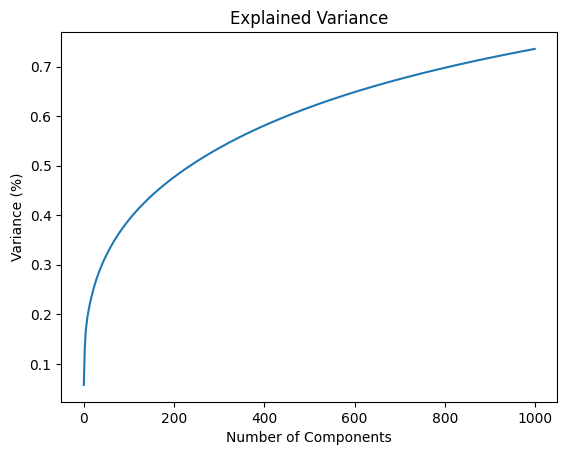
\includegraphics[width=0.73\linewidth]{images/pca_bow.png}
	\end{figure}
}

\pause
\only<4> {
	\vspace{-3mm}
	\begin{figure}[h]
		\caption{t-SNE 300 iterations + PCA to 50 on Bag of Words}
		\centering
		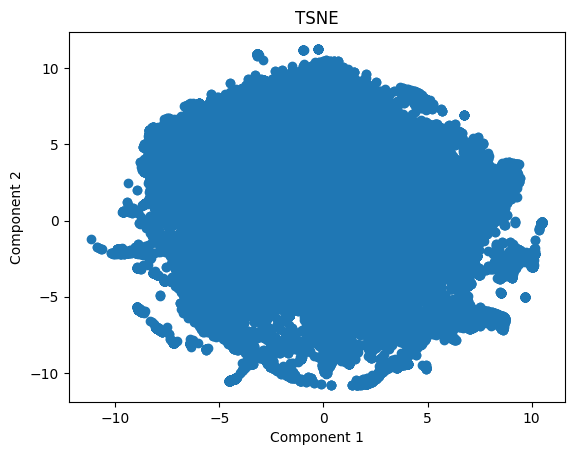
\includegraphics[width=0.73\linewidth]{images/tsne_300_bow.png}
	\end{figure}
}

\end{frame}


\begin{frame}[t]{Models}

\vspace{-3mm}

\begin{itemize}
\item KNN \\
Seemed to be a good baseline for our project, since its so simple

\pause
\item Naive Bayes \\
Also quite simple in practice, but a bit more interesting in the context of text classification

\pause
\item Logistic Regression \\
Classical approach

\pause
\item Decision Trees \\
Do not have the best reputation, so we wanted to check how they perform

\pause
\item Random Forest \\
Natural extension of Decision Trees

\pause
\item Simple perceptron-based neural network \\
It is a neural network, thus we could not skip it

\pause
\item Support Vector Machine \\
Interesting concept
\end{itemize}
\end{frame}

\begin{frame}[t]{Evaluation}

\vspace{-3mm}

Since choosing proper evaluation function is a major part of our project (because we have specific multi-label classification) we decided to use following metrics:
	
\begin{itemize}
	
\pause
\item Exact match \\
typical approach for one label - the prediction must be exact
	
\pause
\item Precision {\it TP/(TP+FP)} \\
we focus on minimizing FP

\pause
\item Recall {\it TP/(TP+FN)} \\
we focus on minimizing FN

\pause
\item F1-score {\it (2 * precision * recall) / (precision + recall)} \\
combines precision and recall

\pause
\item Intersection over union score \\
this evaluation does not treat each label separately, but check ratio of intersection and union
\end{itemize}
\end{frame}


\begin{frame}[t]{Results - KNN}
\only<1> {
	\vspace{-3mm}
	\begin{figure}[h]
		\caption{Different number of neighbors}
		\centering
		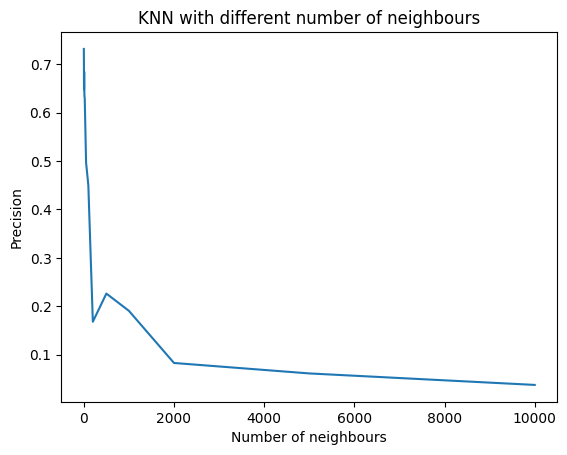
\includegraphics[width=0.73\linewidth]{images/KNN/f1_score_over_k_large.png}
	\end{figure}
}

\pause
\only<2> {
	\vspace{-3mm}
	\begin{figure}[h]
		\caption{Comparison of evaluations}
		\centering
		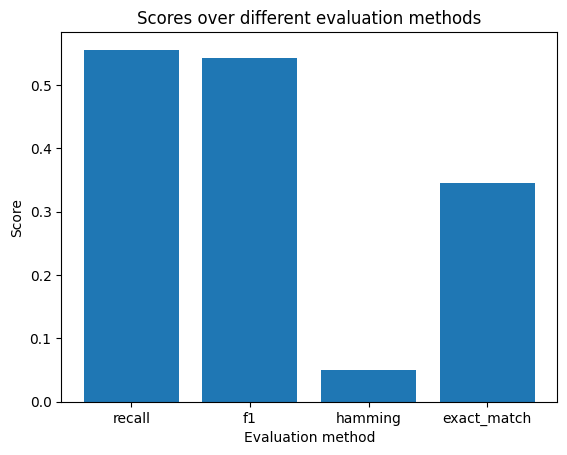
\includegraphics[width=0.73\linewidth]{images/KNN/score_every_eval.png}
	\end{figure}
}
\end{frame}


\begin{frame}[t]{Results - Logistic Regression}
	\vspace{-3mm}
	\begin{figure}[h]
		\centering
		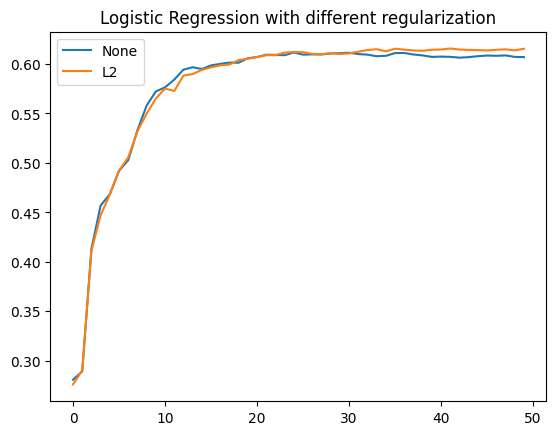
\includegraphics[width=0.8\linewidth]{images/LogisticRegression/none_l2_regularization.png}
	\end{figure}
\end{frame}

% TODO: add precision score	
\begin{frame}[t]{Results - Decision Tree}
\vspace{-3mm}
\begin{figure}[h]
	\centering
	\begin{minipage}{0.3\textwidth}
		\centering
		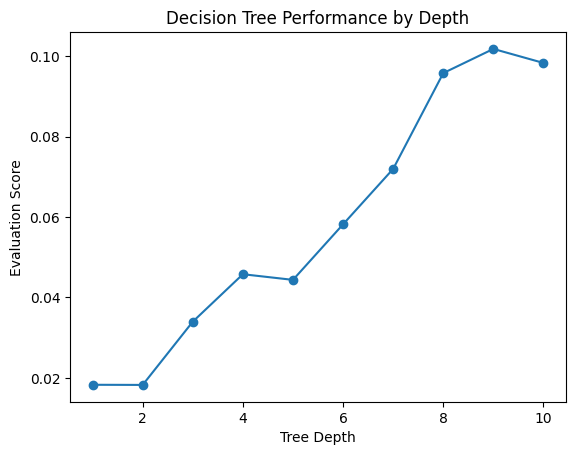
\includegraphics[width=\linewidth]{images/DecisionTree/exactmatch.png}
		\caption{Exact match}
	\end{minipage}
	\hfill
	\begin{minipage}{0.3\textwidth}
		\centering
		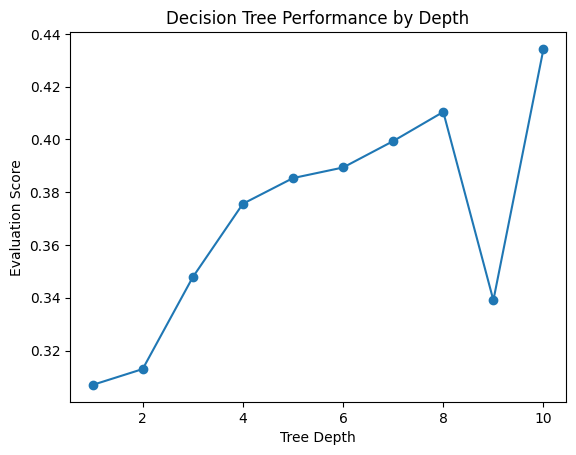
\includegraphics[width=\linewidth]{images/DecisionTree/f1_score.png}
		\caption{F1-score}
	\end{minipage}
	\hfill
	\begin{minipage}{0.3\textwidth}
		\centering
		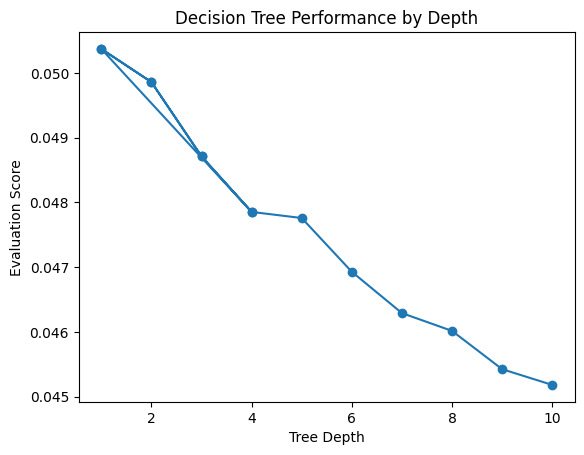
\includegraphics[width=\linewidth]{images/DecisionTree/hammingloss.png}
		\caption{Hamming loss}
	\end{minipage}
	\vfill
	\begin{minipage}{0.3\textwidth}
		\centering
		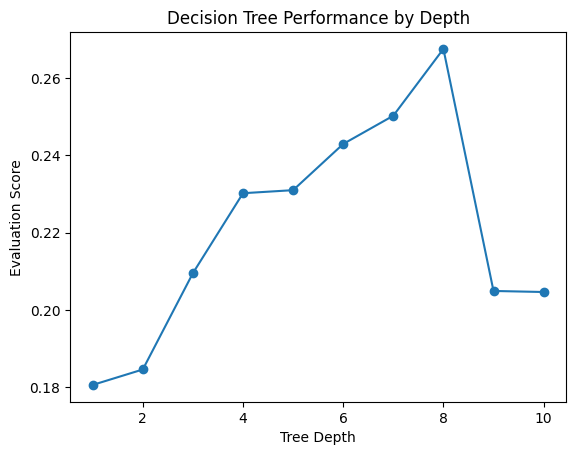
\includegraphics[width=\linewidth]{images/DecisionTree/jaccardscore.png}
		\caption{Intersection}
	\end{minipage}
	\hfill
	\begin{minipage}{0.3\textwidth}
		\centering
		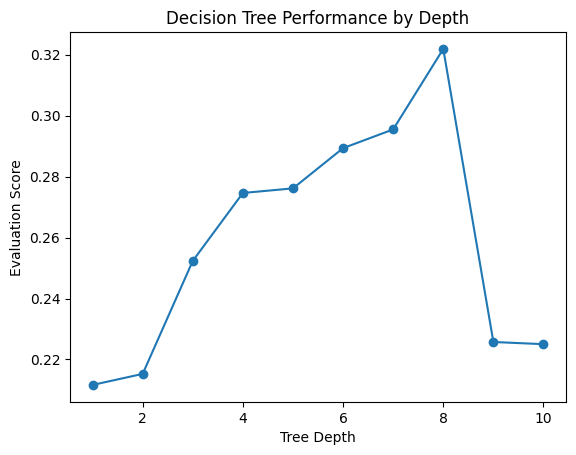
\includegraphics[width=\linewidth]{images/DecisionTree/recall.png}
		\caption{Recall}
	\end{minipage}
\end{figure}
\end{frame}

\begin{frame}[t]{Results - Random Forest}
\only<1>{
	\vspace{-3mm}
	\begin{figure}[h]
		\caption{Different number of trees, no depth limit}
		\centering
		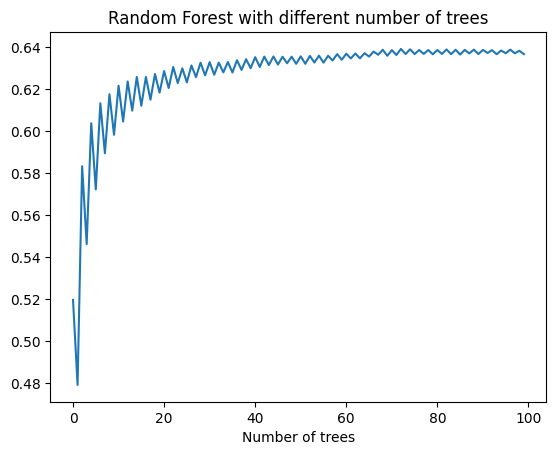
\includegraphics[width=0.73\linewidth]{images/RandomForest/compare_trees_nolimit.png}
	\end{figure}
}

\pause
\only<2>{
	\vspace{-3mm}
	\begin{figure}[h]
		\caption{Different number of trees, depth limited to 100}
		\centering
		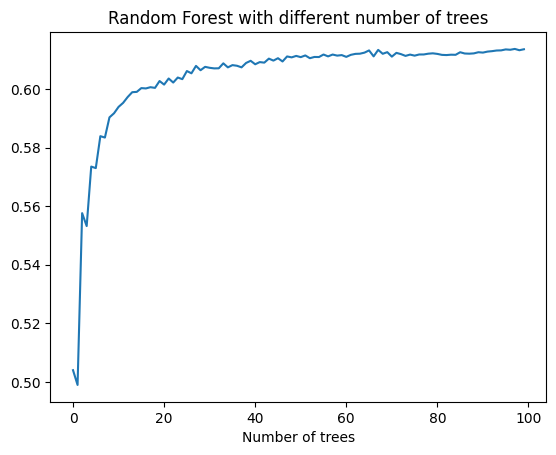
\includegraphics[width=0.73\linewidth]{images/RandomForest/compare_trees_depth100.png}
	\end{figure}
}
\end{frame}

\begin{frame}[t]{Results - Support Vector Machine}
	\vspace{-3mm}
	\begin{figure}[h]
		\centering
		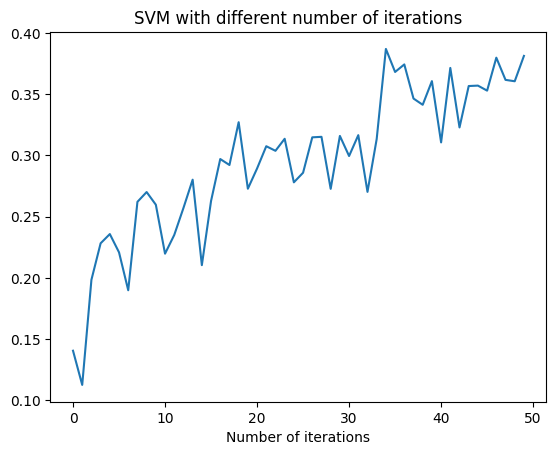
\includegraphics[width=0.8\linewidth]{images/SVM/precision.png}
	\end{figure}
\end{frame}


\begin{frame}[t]{Results - Neural Network}
	\vspace{-3mm}
	\begin{figure}[h]
		\caption{Multilayer Perceptron}
		\centering
		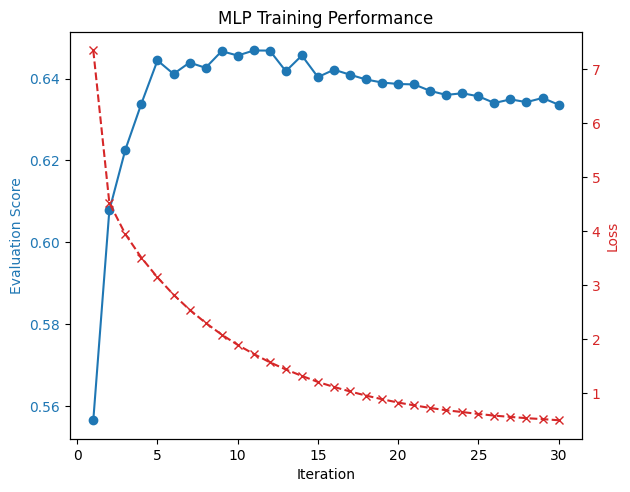
\includegraphics[width=0.73\linewidth]{images/MLP/mlp_over_iters.png}
	\end{figure}
\end{frame}


\begin{frame}[t]{Input preprocessing}
\vspace{-3mm}
\begin{figure}[h]
	\caption{Logistic Regression, F1-score}
	\centering
	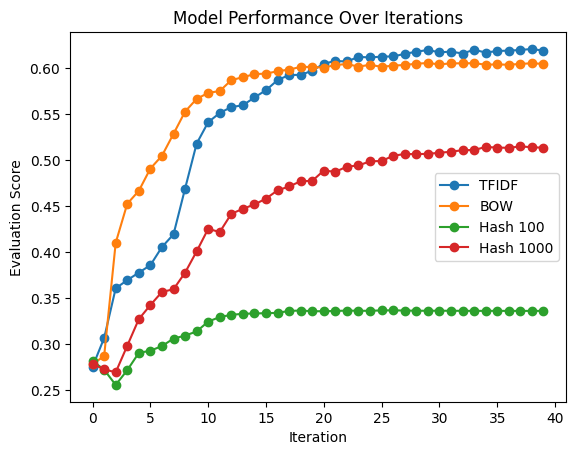
\includegraphics[width=0.73\linewidth]{images/LogisticRegression/f1score_compare_inprep.png}
\end{figure}
\end{frame}


\begin{frame}[t]{Evaluation metrics}
\only<1>{
	\vspace{-3mm}
	\begin{figure}[h]
		\caption{Logistic Regression, F1-score}
		\centering
		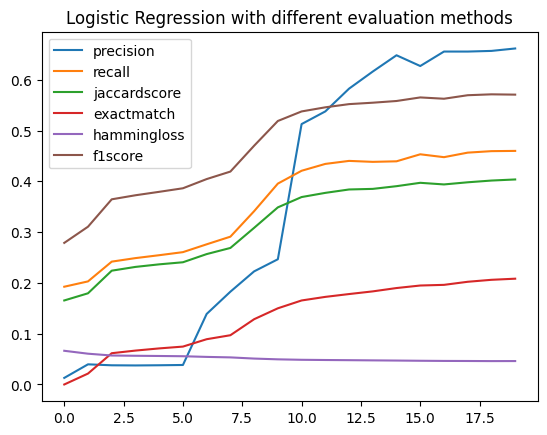
\includegraphics[width=0.73\linewidth]{images/LogisticRegression/compare_evaluations.png}
	\end{figure}
}
\end{frame}	


\begin{frame}[t]{Models Comparison}
	\vspace{-3mm}
	\begin{figure}[h]
		\centering
		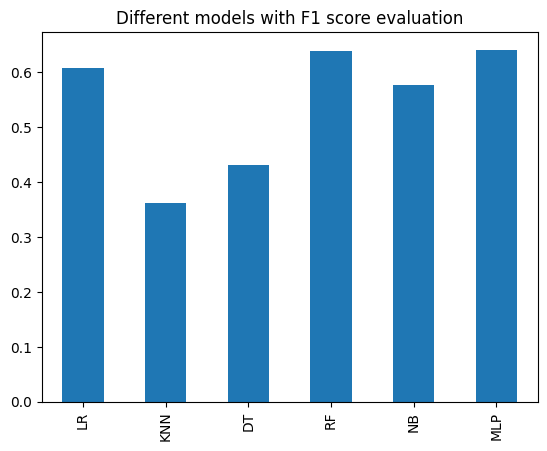
\includegraphics[width=0.8\linewidth]{images/models_comparison.png}
	\end{figure}
\end{frame}

\begin{frame}[t]{Conclusions}
\begin{itemize}[<+->]
	\item From the input preprocessors the most effective was {\bf TF-IDF} \\
	(that makes sense, as it carries the most information)
	\item The best model was {\bf neural network}, with {\bf random forest} and {\bf logistic regression} not far behind \\
	(additionally neural network was the most time consuming to train)
	\item {\bf KNN} indeed was far from beeing the best model \\
	but {\bf naive bayes}, which was the fastest, was quite good
	\item {\bf Decision trees} were empirically proven (again) that they are not the best choice
	\item {\bf SVM} did not perform too bad, nor too good \\
	we suspect that, based on how it works, it could {\bf eventually} perform way better (but that would require a lot of time)
\end{itemize}
\end{frame}

\end{document}